\documentclass[12pt]{myland}

%%% Formatting
\def\<#1>{\texttt{#1}}
\setlength{\parskip}{1em}

%%%%%%%%%%%%%%%%%%%%%%%%%%%%FILE TITLE%%%%%%%%%%%%%%%%%%%%%%%%%%%%%%%%%%%%
\begin{document}
\begin{center}
	{\Large \myhwname{CSE 444: \<SimpleDB> Final Report}} \\
	\vspace{.05in}
    \myname{Linxing Preston Jiang}\quad\quarter{Winter 2018}\\
	\vspace{.05in}
    \today \\
\end{center}
\vspace{.15in} \hrule \vspace{0.5em}%

\section{Overall System Architecture}
	\label{overview}

	\par In a typical database architecture, there are four main components: Process Manager, Query Executor, Share
Utilities, and Storage Manger (Balazinska, Mass, Lecture 3). For our implementation of \<SimpleDB> in the labs,
we focus on the Storage Manager and Query Executor: adding access methods for data store on disk in lab1, adding both file
mutability (insert/delete tuples to/from file system, eviction from full BufferPool) and query operators (SeqScan, Join,
etc.) \& aggregates (min, max, etc.) in lab2, adding lock manager in lab3, adding log manager in lab4, and finally, adding
parallel data processing in lab6.

    Figure \ref{fig:architecture} shows the parts of the architecture of \<SimpleDB> which we implemented in the labs.
    \begin{figure}[h]
        \begin{mybox}
            \begin{tikzpicture}[
            >=latex,shorten >=2pt,shorten <=2pt,shape aspect=1,
        ]
            \tikzstyle{cyl} = [cylinder, shape border rotate=90, draw, minimum height=1cm, minimum width=5cm]
            \tikzstyle{noo} = [rectangle, draw, minimum height=1cm, minimum width=5cm]
            \tikzstyle{cir} = [ellipse, draw, minimum height=1cm, minimum width=2cm]
            \tikzstyle{poi} = [ellipse, draw, fill]
            \tikzstyle{joining} = []
            \tikzset{>=stealth}
            \tikzstyle{readup} = [red, ->]
            \tikzstyle{comm} = [blue, ->]
        % Disk Interface %
        \node[noo, minimum height = 8cm, minimum width = 6cm, dashed] (diski) at (-10, 2) {};
            \node at ($(diski) + (0, 4)$) {Disk Inerface};
        \node[cyl] (disk) at (-10, 0) {Disk};
        \node[noo, minimum height=0.5cm, minimum width=1cm] (diskpage) at (-10, 0.8) {\<File f>};
        \node (diskpage1) at (diskpage.north east) {};
        \node (diskpage2) at (diskpage.north west) {};
        % Heapfile
        \node[noo, minimum height=3cm, minimum width=5cm] (heapfile) at (-10, 3.7) {};
            \node at (heapfile.north) {HeapFile};
        \node (heapfile1) at (heapfile.south east) {};
        \node (heapfile2) at (heapfile.south west) {};
        \path[->] (diskpage1) edge (heapfile1);
        \path[->] (diskpage2) edge (heapfile2);
        % Heappage
        \node[noo, minimum height=1.5cm, minimum width=1cm] (heappage) at (-12, 3.2) {};
        \node[noo, minimum height=1.5cm, minimum width=1cm] (heappage2) at (-11, 3.2) {};
            \node at ($(heappage2.north) + (-0.5, 0)$) {\small{HeapPage}};
            \node at ($(heappage2) + (1, 0)$) {...};
        % Tuple
        \node[noo, minimum height=.1cm, minimum width=.2cm] (tuple1) at (-12.35, 3) {};
        \node[noo, minimum height=.1cm, minimum width=.2cm] (tuple2) at (-12.15, 3) {};
        \node[noo, minimum height=.1cm, minimum width=.2cm] (tuple3) at (-11.95, 3) {};
            \node at (-12.15, 3.5) {\small{Tuple}};
            \node at (-11.75, 3) {...};
        \node (meta) at ($(heapfile)+ (0.5, 0)$) {metadata};

        % Execution Interface
        \node[noo, minimum height=3cm, minimum width=2cm] (buffer) at ($(heapfile) + (6, -3)$) {BufferPool};
        \node[noo, minimum height=1cm, minimum width=2cm] (lock) at ($(buffer)+ (0, 4.5)$) {Lock Manager};
        \node[noo, minimum height=1cm, minimum width=2cm] (log) at ($(lock)+ (0, -1.5)$) {Log Manager};
        \node[noo, minimum height=1.5cm, minimum width=2cm] (catalog) at ($(buffer)+ (0, -3)$) {Catalog};
        \node[noo, minimum height=10cm, minimum width=4cm, dashed] (storage) at ($(buffer)+ (0, 0.5)$) {};
            \node at ($(storage) + (0, 5)$) {Storage Manager};
        % Executor
        \node[noo, minimum height=4.5cm, minimum width=5.5cm, dashed] (exec) at ($(log) + (5, 0.6)$) {};
        \node[noo, minimum height=1cm, minimum width=2cm] (it) at ($(log) + (4, -1)$) {\small{IteratorInterface}};
            \node at ($(it) + (1, -1)$)  {\small{Query Executor}};
        \node (it1) at ($(it) + (3, 1)$) {\tiny{SeqScan}};
        \node (it2) at ($(it1) + (0, 0.5)$) {\tiny{Join}};
        \node (it3) at ($(it2) + (0, 0.5)$) {\tiny{Filter}};
        \node (it4) at ($(it3) + (0, 0.5)$) {\tiny{Aggregates}};
        \node (it5) at ($(it4) + (0, 0.5)$) {\tiny{...}};
        \foreach \x in {1, 2, 3, 4, 5} {
            \path[->] (it) edge [bend left = \x0] (it\x);
        }
    \end{tikzpicture}

        \end{mybox}
       \caption{\<SimpleDB> Architecture}
        \label{fig:architecture}
    \end{figure}

    \subsection{\<BufferPool> and \<Opertors>}
        BufferPool is responsible for both caching pages in memory that have been recently read
        from disk and handle concurrency and transactions. All operators read and write pages from various files
        on disk through the buffer pool. Operators are responsible for executing query plans. In \<SimpleDB>, each operator
        implements the \<OpIterator> interface, which supports \<open, hasNext, next, rewind, > and
        \<close>. Operators are connected together into a plan by passing lower-level operators into the
        constructors of higher-level operators (Lab1 ReadMe). Programs call \<next> on the root operator and then
        fetch tuples recursively through the plan tree in one pass top-down and another pass bottom-up. \par


    \begin{figure}[t!]
        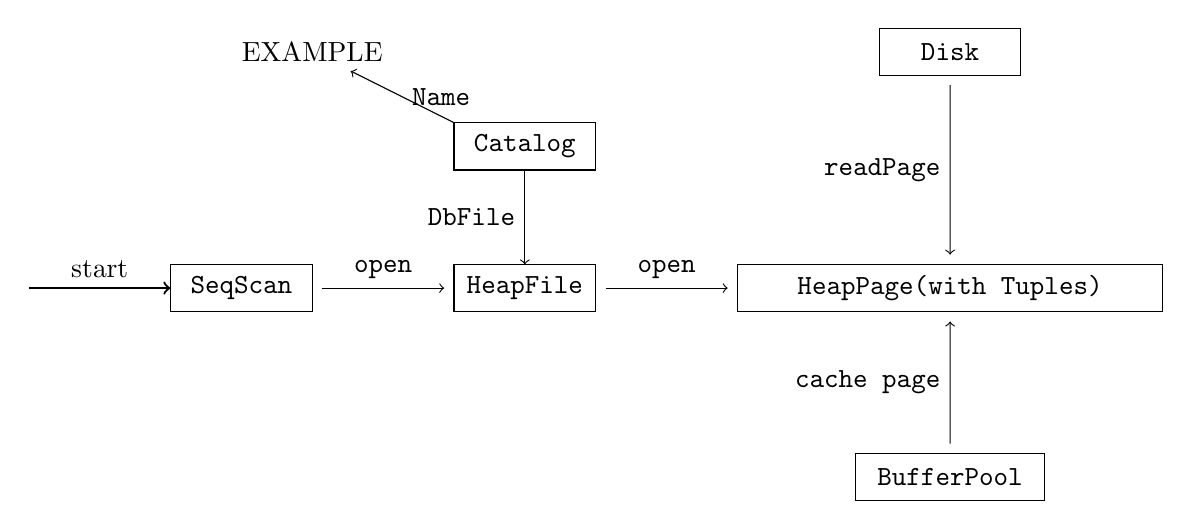
\begin{tikzpicture}[
            scale=.6,
        ]
            \path[->, thick] (-3, -0.5) edge node[midway, above] {start} (0, -0.5);
            \draw[draw=black] (0, 0) rectangle (3, -1) node[midway]  {\texttt{SeqScan}};
            \node (seq) at (3, -0.5) {};
            \draw[draw=black] (6, 0) rectangle (9, -1) node[midway] {\texttt{HeapFile}};
            \node (heapfilel) at (6, -0.5) {};
            \node (heapfiler) at (9, -0.5) {};
            \path[->] (seq) edge node[midway, above] {\texttt{open}} (heapfilel);
            \draw[draw=black] (12, 0) rectangle (21, -1) node[midway] {\texttt{HeapPage(with Tuples)}};
            \node (pagel) at (12, -0.5) {};
            \node (pager) at (21, -0.5) {};
            \node (pageu) at (16.5, 0) {};
            \node (paged) at (16.5, -1) {};
            \path[->] (heapfiler) edge node[midway, above] {\texttt{open}} (pagel);
            \draw[draw=black] (15, 5) rectangle (18, 4) node[midway] {\texttt{Disk}};
            \node (disk) at (16.5, 4) {};
            \path[->] (disk) edge node[midway, left] {\texttt{readPage}} (pageu);
            \draw[draw=black] (14.5, -5) rectangle (18.5, -4) node[midway] {\texttt{BufferPool}};
            \node (buffer) at (16.5, -4) {};
            \path[->] (buffer) edge node[midway, left] {\texttt{cache page}} (paged);
            % catalog
            \draw[draw=black] (6, 3) rectangle (9, 2) node[midway] {\texttt{Catalog}};
            \path[->] (7.5, 2) edge node[midway, left] {\texttt{DbFile}} (7.5, 0);
            \node (name) at (3, 4.5) {EXAMPLE};
            \path[->] (6, 3) edge node[midway, right] {\texttt{Name}} (name);
        \end{tikzpicture}
        \caption{\<SimpleDB> \texttt{open}}
        \label{fig:open}
    \end{figure}

    \begin{figure}[h!]
        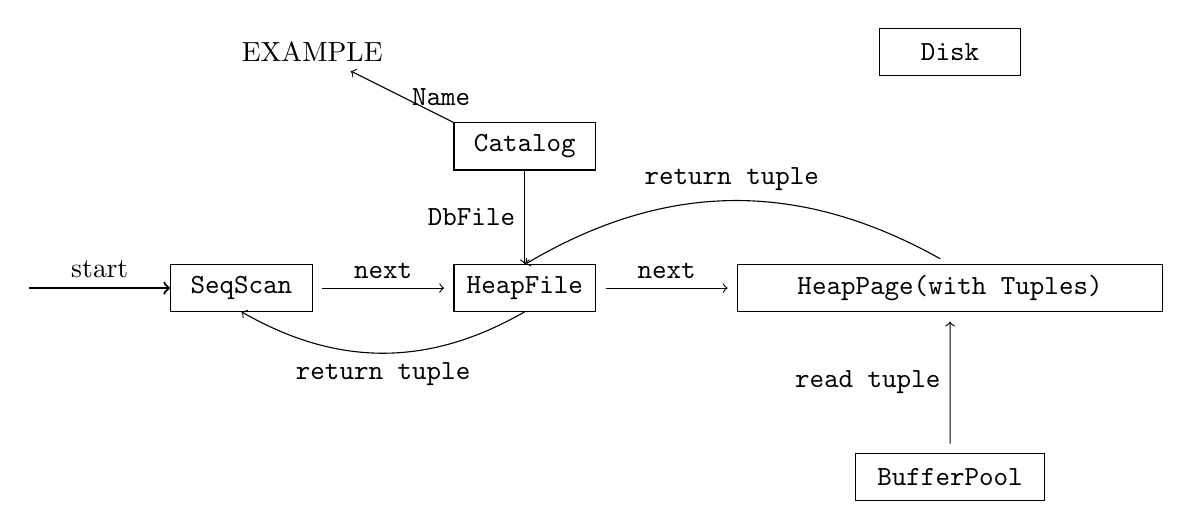
\begin{tikzpicture}[
            scale=.6,
        ]
            \path[->, thick] (-3, -0.5) edge node[midway, above] {start} (0, -0.5);
            \draw[draw=black] (0, 0) rectangle (3, -1) node[midway]  {\texttt{SeqScan}};
            \node (seq) at (3, -0.5) {};
            \draw[draw=black] (6, 0) rectangle (9, -1) node[midway] {\texttt{HeapFile}};
            \node (heapfilel) at (6, -0.5) {};
            \node (heapfiler) at (9, -0.5) {};
            \path[->] (seq) edge node[midway, above] {\texttt{next}} (heapfilel);
            \draw[draw=black] (12, 0) rectangle (21, -1) node[midway] {\texttt{HeapPage(with Tuples)}};
            \node (pagel) at (12, -0.5) {};
            \node (pager) at (21, -0.5) {};
            \node (pageu) at (16.5, 0) {};
            \node (paged) at (16.5, -1) {};
            \path[->] (heapfiler) edge node[midway, above] {\texttt{next}} (pagel);
            \draw[draw=black] (15, 5) rectangle (18, 4) node[midway] {\texttt{Disk}};
            \node (disk) at (16.5, 4) {};
            \draw[draw=black] (14.5, -5) rectangle (18.5, -4) node[midway] {\texttt{BufferPool}};
            \node (buffer) at (16.5, -4) {};
            \path[->] (buffer) edge node[midway, left] {\texttt{read tuple}} (paged);
            \path[->] (pageu) edge [bend right] node[midway, above] {\texttt{return tuple}} (7.5, 0) ;
            \path[->] (7.5, -1) edge [bend left] node[midway, below] {\texttt{return tuple}} (1.5, -1) ;
            \draw[draw=black] (6, 3) rectangle (9, 2) node[midway] {\texttt{Catalog}};
            \path[->] (7.5, 2) edge node[midway, left] {\texttt{DbFile}} (7.5, 0);
            \node (name) at (3, 4.5) {EXAMPLE};
            \path[->] (6, 3) edge node[midway, right] {\texttt{Name}} (name);
        \end{tikzpicture}
        \caption{\texttt{SimpleDB} \texttt{next}}
        \label{fig:next}
    \end{figure}
        In Lab 1, we implemented \<getPage> which is needed for reading Pages into memory and getting tuples,
        together with \<SeqScan> operator to scan the file and return tuples. The workflow of opening opertators
        to read file and caching pages into BufferPool is shown by Figure \ref{fig:open}, and the workflow of recursively
        getting tuples through \<SeqScan> using \<next()> is shown by Figure \ref{fig:next}. \par

        In Lab 2, We added \<insert>, \<delete> funcionalities in \<SimpleDB>, which insert/delete tuples to/from the
        pages in BufferPool by calling the method from \<HeapFile> to update the page, then \<BufferPool>
        updates the records by re-inserting the pages into the \<BufferPool>. When the \<BufferPool> is
        full and a new page need adding, \<writePage> from \<HeapFile> will be called to write the dirty
        page to disk and add the new page into the \<BufferPool>. \<BufferPool> is in charge of updating
        the pages because \<Insert/Delete> operators directly call \<insert/delete> of \<BufferPool>. Besides, we also
        implemented \<Filter>, \<Join> operators and the aggregates. As an example, Figure \ref{fig:join} shows the
        workflow of using \<Join> opeator and Figure \ref{fig:insert} shows the workflow of inserting tuples.

        \begin{figure}[htb!]
            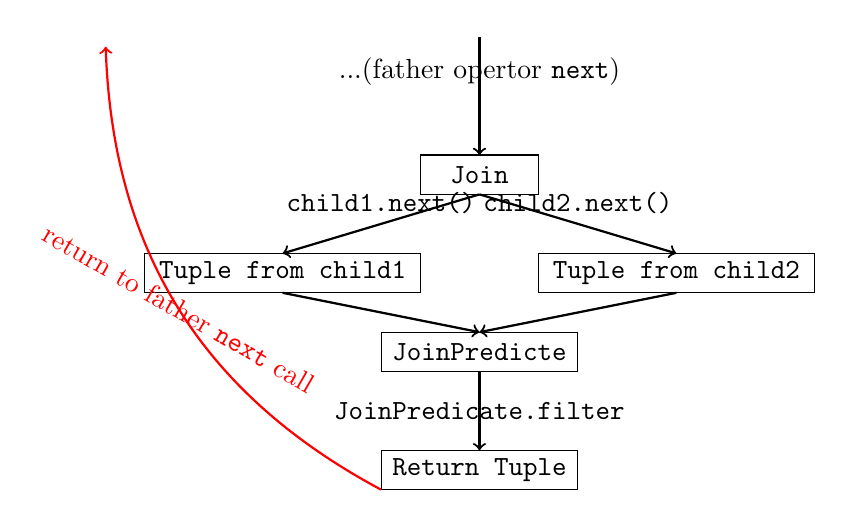
\begin{tikzpicture}[
                scale=.5,
            ]
                \path[->, thick] (3, 3) edge node[midway, above] {...(father opertor \texttt{next})} (3, 0);
                \draw[draw=black] (1.5, 0) rectangle (4.5, -1) node[midway]  {\texttt{Join}};
                \path[->, thick] (3, -1) edge node[midway, above] {\texttt{child1.next()}} (-2, -2.5);
                \path[->, thick] (3, -1) edge node[midway, above] {\texttt{child2.next()}} (8, -2.5);
                \draw[draw=black] (-5.5, -2.5) rectangle (1.5, -3.5) node[midway]  {\texttt{Tuple from \texttt{child1}}};
                \draw[draw=black] (4.5, -2.5) rectangle (11.5, -3.5) node[midway]  {\texttt{Tuple from \texttt{child2}}};
                \path[->, thick] (-2, -3.5) edge node[midway, above] {} (3, -4.5);
                \path[->, thick] (8, -3.5) edge node[midway, above] {} (3, -4.5);
                \draw[draw=black] (0.5, -4.5) rectangle (5.5, -5.5) node[midway]  {\texttt{JoinPredicte}};
                \path[->, thick] (3, -5.5) edge node[midway] {\texttt{JoinPredicate.filter}} (3, -7.5);
                \draw[draw=black] (0.5, -7.5) rectangle (5.5, -8.5) node[midway]  {\texttt{Return Tuple}};
                \node (father) at (-6.5, 3) {};
                \path[->, thick, color=red] (0.5, -8.5) edge [bend left=30] node[midway, rotate=330] {return to father \texttt{next} call} (father);
            \end{tikzpicture}
            \caption{\<SimpleDB join>}
            \label{fig:join}
        \end{figure}

    \subsection{Lock Manager}
    Lab 3 focuses on adding Transactions functionality to simpleDB. In order to achieve this, we implemented our own
    \texttt{Lock} and \texttt{LockManager} which together handle acquiring/releasing both \texttt{SHARED} (read-only)
    and \texttt{EXCLUSIVE} (read-write) locks by different transactions on page granularity. \<SimpleDB> uses time-
    out limits for \texttt{acquire} so that a certain period time of blocking on \texttt{acquire} will be considered as
    deadlock and thus abort the transaction. \par

    \begin{figure}[htb!]
        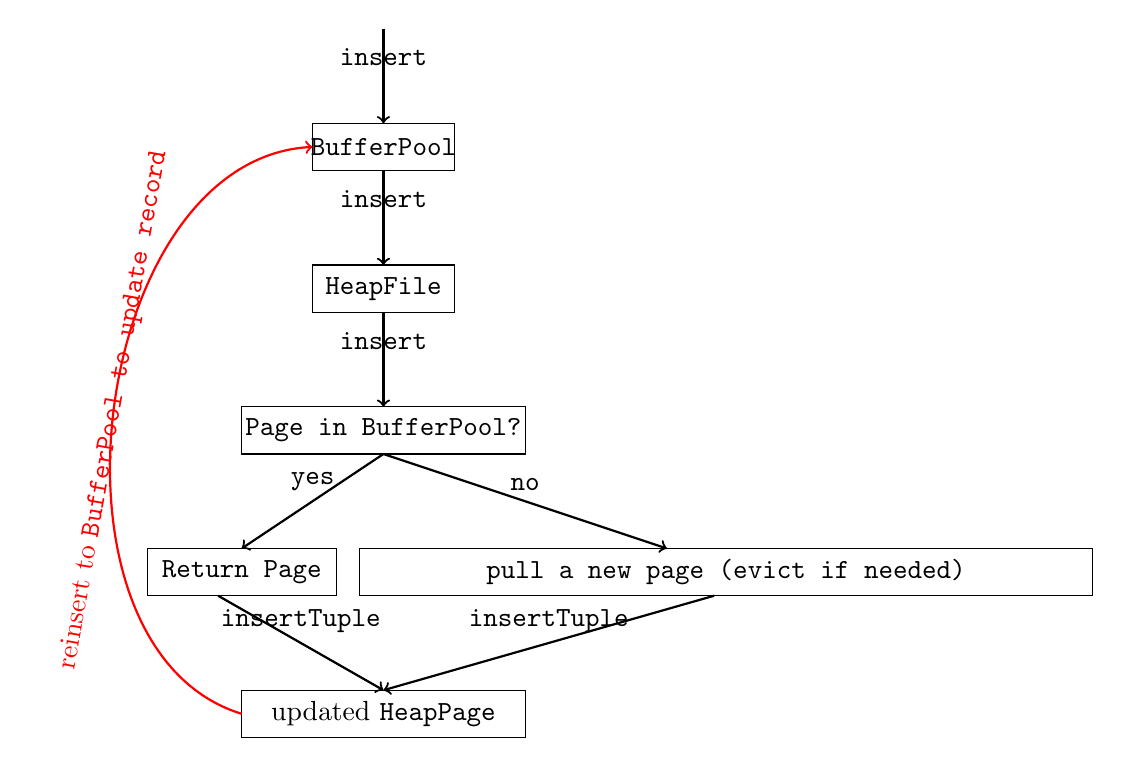
\begin{tikzpicture}[
            scale=.6,
        ]
            \path[->, thick] (0, 2) edge node[midway, above] {\texttt{insert}} (0, 0);
            \draw[draw=black] (-1.5, 0) rectangle (1.5, -1) node[midway]  {\texttt{BufferPool}};
            \path[->, thick] (0, -1) edge node[midway, above] {\texttt{insert}} (0, -3);
            \draw[draw=black] (-1.5, -3) rectangle (1.5, -4) node[midway]  {\texttt{HeapFile}};
            \path[->, thick] (0, -4) edge node[midway, above] {\texttt{insert}} (0, -6);
            \draw[draw=black] (-3, -6) rectangle (3, -7) node[midway]  {\texttt{Page in BufferPool?}};
            \path[->, thick] (0, -7) edge node[midway, above] {\texttt{yes}} (-3, -9);
            \path[->, thick] (0, -7) edge node[midway, above] {\texttt{no}} (6, -9);
            \draw[draw=black] (-5, -9) rectangle (-1, -10) node[midway]  {\texttt{Return Page}};
            \draw[draw=black] (-0.5, -9) rectangle (15, -10) node[midway]  {\texttt{pull a new page (evict if needed)}};
            \path[->, thick] (-3.5, -10) edge node[midway, above] {\texttt{insertTuple}} (0, -12);
            \path[->, thick] (7, -10) edge node[midway, above] {\texttt{insertTuple}} (0, -12);
            \draw[draw=black] (-3, -12) rectangle (3, -13) node[midway]  {updated \texttt{HeapPage}};
            \path[->, thick, color=red] (-3, -12.5) edge [bend left=80] node[midway, rotate=80] {reinsert to \texttt{BufferPool
                to update record}} (-1.5, -0.5);
        \end{tikzpicture}
        \caption{\<SimpleDB insertTuple>}
        \label{fig:insert}
    \end{figure}

	\begin{itemize}
        \item \texttt{Lock}: We need this class to represent the two types of locks simpleDB uses: \texttt{SHARED} and
            \texttt{EXCLUSIVE}. A shared lock is acquired by read-only transactions, and thus can be shared between
            many read-only transactions; an exclusive lock is acquired by read-write transactions, and thus can only be
            acquired by at most one read-write transaction at a time.
        \item \texttt{LockManager}: We need this class as the manager for all locking-related actions in simpleDB. It
            is created within \texttt{BufferPool} and will be called to acquire locks when \texttt{getPage} is called
            and release locks when \texttt{transactionComplete} is called. Note that because of the design of simpleDB,
            \texttt{acquire} in \texttt{LockManager} should only need calling in \texttt{getPage} when simpleDB wants to
            interact with a page. There are a few conditions when \texttt{acquire} will not be a blocking call. They are:
                \begin{itemize}
                    \item When the lock on that page is not locked.
                    \item When the lock is locked by this transaction itself (will upgrade a share lock to
                        exclusive if this transaction is the only one which holds the lock)
                    \item When the lock is locked, but it is a shared lock, and the transaction wants a shared lock.
                \end{itemize}
        \item \texttt{BufferPool.transactionComplete}: We add this method to release all locks acquired by a
            transaction when it commits.
	\end{itemize}

    \subsection{Log Manager}
    In Lab 4, we focus on adding rollback and recovery functionality to simpleDB upon abort and system crash.
    Specifically, we implemented STEAL (dirty pages may be evicted from the buffer pool even though the transaction
    hasn't commited yet), and NO FORCE (on transaction commit, no need to force write dirty pages to disk) for buffer
    pool management. In order to achieve this, we implemented log-based rollback and recovery which performs a
    redo-phase and an undo-phase. \par

    \<SimpleDB> supports six kinds of logs: \<BEGIN, COMMIT, ABORT, UPDATE, CHECKPOINT,> and \<CLR>. CLR is part of my
    design in order to make undo-phase easier to implement.

    \begin{itemize}
        \item \texttt{LogFile.rollback}: We need this method to roll back changes made by an aborted transaction. This
        methdo will read from the end of the log file and undo changes made by this transaction until its first active
        log record. It is also implemented that undo changes will append new CLR logs. More of this in the design part
        of this writeup.

        \item \texttt{LogFile.recover}: We need this method to recover a simpleDB system upon unexpected crashes. It
        will start redoing from the beginning of the log file or the last checkpoint log if any, during which a map of
        active transactions to their first active log line is built. Then, undo-phase will use the active transaction
        map and undo any changes made by these transactions bottom up.
	\end{itemize}

\section{Parallel Data Processing}
	\label{parallel}

    In Lab 6, we added the ability of parallel data processing to \<SimpleDB>. The basic structure of parallel \<SimpleDB>
    contains \<Worker> and \<Server>. The workflow goes as follows: for every query users enter, it is first sent to
    \<Server> for some optimization (we did not implement this part this quarter). Next step is to prepare this query to
    be run in parallel by inserting new operators (more on this later). The this query will be sent to all
    available workers. After each worker receives the query, it will localize it (more on this later) and run the query.
    Finally, each worker will send the results back to \<Server>, then server will aggregate all the results and send
    the final result back to users. \par

    Our implementation of parallel \<SimpleDB> focuses on the following subparts of implementing a functional model:
    \begin{itemize}
        \item How to localize a query to run it on a local machine? (\<Worker.java>)
        \item How to transfer data in between workers? (\<ShuffleProducer.java> \& \<ShuffleConsumer.java>)
        \item How to optimize aggregate performance in a parallel setting? (\<AggreagateOptimizer.java>)
    \end{itemize}
    The following sections explain the detailed implementations on these questions.

    \subsection{\<Worker.java>}
    In \<Worker.java>, we localize the query for it to run on the local machine. It does three jobs: (1) For \<SeqScan>
    operators, we reset its \<tid> and \<alias>. This is because the \<tid> of the \emph{local} table may not be the
    same as the one of global table, and the \<Catalog> is a local verlsion. We need to update the \<tid> so that
    \<SeqScan> reads the correct subtable; (2) For \<Producers>, we set its worker to \<this>. This is because \<Worker>
    handles the data buffer of \<Consumers> (more on this later) and the \<Producer> needs to know which bufffer to send
    data to for the \<Consumer> to get data; (3) For \<Consumers>, we set its data buffer in \<Worker> through its
    \<inBuffer> map.

    \subsection{\<ShuffleProducer.java> \& \<ShuffleConsumer.java>}
    We implement \<ShuffleProducer.java> \& \<ShuffleConsumer.java> to enable data transfer between workers. In
    \<ShuffleProducer.java>, in order to handle multiple connections with multiple \<ShuffleConsumer> (whose addresses
    are stored in a \<SocketInfo> wrapper), we keep three lists of \<IoSession> as connections, \<List> as data buffers,
    and \<Long> as timestamps, one combination for one \<Consumer>.




\section{Discussion}
	\label{discussion}
\end{document}
